\documentclass[a4paper,10pt]{book} %type de document et paramètres


\usepackage[utf8]{inputenc} %package fondamental
\usepackage[T1]{fontenc} %package fondamental
\usepackage[english,francais]{babel} %package de langues
\usepackage{lmodern} %police de caractère

\usepackage[top=3cm, bottom=3cm, left=4cm, right=2cm]{geometry} %permet de paramétrer les marges par défaut
\usepackage{changepage} %permet de modifier localement une mise en page (marges,...) : utilisé pour la page de garde
\usepackage{multicol} %permet de mettre plusieurs colonnes (\begin{multicols}{2} \end{multicols} jusqu'à 10 colonnes)
\usepackage[pdftex, pdfauthor={Pierre Gimalac}, pdftitle={Physique II}, pdfsubject={Physique}, pdfkeywords={Physique, Mécanique, Mathématiques}, colorlinks=true, linkcolor=black]{hyperref} %permet de se déplacer dans le pdf depuis le sommaire en cliquant sur les titres, ainsi que de parametrer les meta données du PDF
\usepackage{url} %permet de mettre des URL actifs \url{}
\let\urlorig\url
\renewcommand{\url}[1]{\begin{otherlanguage}{english}\urlorig{#1}\end{otherlanguage}}

\usepackage{mathtools,amssymb,amsthm} %maths
\usepackage{mathrsfs} %maths (par exemple les lettres caligraphiées)
\usepackage{stmaryrd} %maths (par exemple les ensembles d'entiers)
\usepackage{calrsfs} %maths (par exemple les notations des ensembles)
\usepackage{xlop} %permet d'afficher des opérations mathématiques
\usepackage[squaren,Gray]{SIunits} %permet de noter des unités proprement
\usepackage{esdiff} %permet d'écrire la dérivée avec la notation de Leibniz \diff{v}{t}

\usepackage{graphicx} %permet d'insérer des images proprement (ajoute des parametres)
\usepackage{wrapfig} %permet de mettre des images à coté d'un texte
%\usepackage{pdfpages} %permet d'insérer un pdf \includepdf[pages={1-2}]{truc.pdf}
%\usepackage{ulem} %permet de souligner/barrer du texte
%\usepackage{soul} %permet de souligner/barrer du texte
\usepackage{cancel} %permet de barrer du texte /cancel{text}
\usepackage{enumitem}

\usepackage{tikz} %package trooop bien permet de dessiner tout et n'importe quoi ! \begin{tikzpicture}
%\usepackage{circuitikz} %permet de dessiner des circuits logiques (entre autre) avec la syntaxe de tikz (\begin{circuitikz}) par exemple \node[american not port] pour le 'non'


%\newcommand{\R}{\mathbb{R}}
%\newcommand{\Rpe}{\mathbb{R}_{+}^{*}}
%\newcommand{\N}{\mathbb{N}}
%\newcommand{\Z}{\mathbb{Z}}
%\newcommand{\C}{\mathbb{C}}
%\newcommand{\Q}{\mathbb{Q}}

\begin{document}

\begin{titlepage}
\newgeometry{margin=2.7cm}
\thispagestyle{empty}
\begin{center}
\vspace*{7cm}
\Huge \textsc{Physique II}\\
\vspace{1.5cm}
\Large Pierre Gimalac\\
\vspace{0.5cm}
\large \textit{Licence de Mathématiques}
\vfill
\end{center}
\large \textit{Janvier - Mai 2017}
\hfill 
\large Cours de José Halloy
\restoregeometry
\end{titlepage}

\renewcommand{\contentsname}{Sommaire}
\thispagestyle{empty}
\tableofcontents
\thispagestyle{empty}

\section*{Préambule}
Ce cours est une suite du cours de \textit{Physique I}, c'est pourquoi tout ce qui nous a été présenté dans ce cours ne figure pas dans ce pdf, seuls les points nouveaux ou étudiés plus en détail seront abordés.

\chapter{Position, mouvement, cinématique}
\section{Repère polaire}
\subsection{Définition}
Le repère polaire est un repère en deux dimensions doté d'un centre $O$, d'un axe dirigé par un vecteur $\overrightarrow{U_R}$ orienté vers le système étudié et d'un axe perpendiculaire au premier de vecteur directeur $\overrightarrow{U_\theta}$. On l'utilise en association avec un repère cartésien $(0,\overrightarrow{i},\overrightarrow{j})$.

\begin{wrapfigure}[9]{r}{5.5cm} 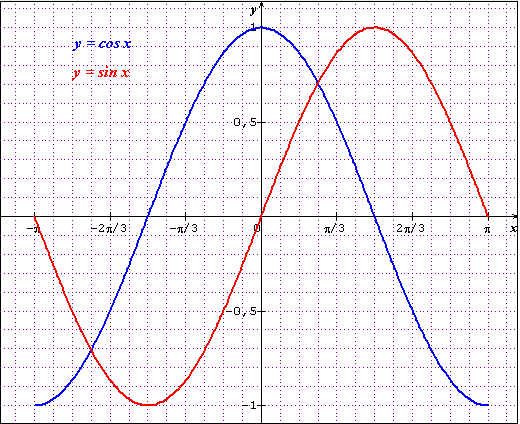
\includegraphics[scale=0.5]{images/001.png} \end{wrapfigure}

\subsection{Coordonnées}

On utilise l'axe des $x$ du repère cartésien pour déterminer un angle $\theta(t)$ entre celui ci et l'axe dirigé par $\overrightarrow{U_R}$ et $\theta+\frac{\pi}{2}$ entre celui-ci et l'axe dirigé par $\overrightarrow{U_\theta}$, et on appelle $R(t)$ la distance entre le système M étudié et le centre O du repère. \\

On a donc $\overrightarrow{U_R}=\cos(\theta)\overrightarrow{i}+\sin(\theta)\overrightarrow{j}$ et\\
$\overrightarrow{U_\theta}=\cos(\theta+\frac{\pi}{2})\overrightarrow{i}+\sin(\theta+\frac{\pi}{2})\overrightarrow{j}= \cos(\theta)\overrightarrow{j}-\sin(\theta)\overrightarrow{i}$.\\\\

$\diff{\overrightarrow{U_R}(t)}{t}=\dot{\theta}(t)(\cos(\theta(t))\overrightarrow{j}-\sin(\theta(t))\overrightarrow{i})=\dot{\theta}(t)\overrightarrow{U_\theta}(t)$

$\diff{\overrightarrow{U_\theta}(t)}{t}=\dot{\theta}(t)(-\cos(\theta(t))\overrightarrow{i}-\sin(\theta(t))\overrightarrow{i})=-\dot{\theta}(t)\overrightarrow{U_\theta}(t)$.

\subsection{Position}
$\overrightarrow{OM}(t)=R(t)\overrightarrow{U_R}(t)=R(t)\cos(\theta(t))\overrightarrow{i}+R(t)\sin(\theta(t))\overrightarrow{j}$.

\subsection{Vitesse}
$\overrightarrow{v}(t)=\diff{\overrightarrow{OM}(t)}{t}=\diff{R(t)\overrightarrow{U_R}(t)}{t}=\dot{R}(t)\overrightarrow{U_R}(t)+R(t)\dot{\theta}(t)\overrightarrow{U_\theta}(t)$.

\subsection{Accélération}
$\overrightarrow{a}(t)=\diff{\overrightarrow{v}(t)}{dt}=\diff{(\dot{R}(t)\overrightarrow{U_R}(t)+R(t)\dot{\theta}(t)\overrightarrow{U_\theta}(t))}{t}$\\

$\phantom{\overrightarrow{a}(t)}=\ddot{R}(t)\overrightarrow{U_R}(t)+\dot{R}(t)\dot{\theta}(t)\overrightarrow{U_\theta}(t)+\dot{R}(t)\dot{\theta}(t)\overrightarrow{U_\theta}(t)+R(t)\ddot{\theta}(t)\overrightarrow{U_\theta}(t)-R(t)\dot{\theta}^2(t)\overrightarrow{U_R}(t)$\\

$\phantom{\overrightarrow{a}(t)}=(\ddot{R}(t)-R(t)\dot{\theta}(t)^2)\overrightarrow{U_R}(t)+(R(t)\ddot{\theta}(t)+2\dot{R(t)}\dot{\theta}(t))\overrightarrow{U_\theta}(t)$.

\newpage

\section{Repère cylindrique}
\subsection{Définition}
Le repère cylindrique est un repère polaire doté un axe vertical de vecteur directeur $\overrightarrow{k}$.

\subsection{Coordonnées}
Les coordonnées sont les mêmes que dans le repère cylindrique avec une coordonnée z en plus.
La coordonnée $R(t)$ correspond ici à la distance entre l'origine $O$ et le projeté orthonormal de $M$ dans le plan défini par les vecteurs $\overrightarrow{i}$ et $\overrightarrow{j}$.

\begin{center} 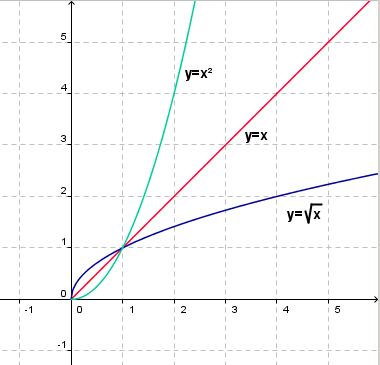
\includegraphics[scale=0.45]{images/002.png} \end{center}

\subsection{Position}
$\overrightarrow{OM}(t)=R(t)\cos(\theta(t))\overrightarrow{i}+R(t)\sin(\theta(t))\overrightarrow{j}+z(t)\overrightarrow{k}$.

\subsection{Vitesse}
$\overrightarrow{v}(t)=\diff{\overrightarrow{OM}(t)}{t}=\diff{(R(t)\overrightarrow{U_R}(t)+z(t)\overrightarrow{k})}{t}=\dot{R}(t)\overrightarrow{U_R}(t)+R(t)\dot{\theta}(t)\overrightarrow{U_\theta}(t)+\dot{z}(t)\overrightarrow{k}$.

\subsection{Accélération}
$\overrightarrow{a}(t)=\diff{\overrightarrow{v}(t)}{t}=\diff{(\dot{R}(t)\overrightarrow{U_R}(t)+R(t)\dot{\theta}(t)\overrightarrow{U_\theta}(t)+\dot{z}(t)\overrightarrow{k})}{t}$\\

$\phantom{\overrightarrow{a}(t)}=\ddot{R}(t)\overrightarrow{U_R}(t)+\dot{R}(t)\dot{\theta}(t)\overrightarrow{U_\theta}(t)+\dot{R}(t)\dot{\theta}(t)\overrightarrow{U_\theta}(t)+R(t)\ddot{\theta}(t)\overrightarrow{U_\theta}(t)-R(t)\dot{\theta}^2(t)\overrightarrow{U_R}(t)+\ddot{z}(t)\overrightarrow{k}$\\

$\phantom{\overrightarrow{a}(t)}=(\ddot{R}(t)-R(t)\dot{\theta}(t)^2)\overrightarrow{U_R}(t)+(R(t)\ddot{\theta}(t)+2\dot{R(t)}\dot{\theta}(t))\overrightarrow{U_\theta}(t)+\ddot{z}(t)\overrightarrow{k}$.

\newpage

\section{Repère sphérique}
\subsection{Définition}
Le repère sphérique est un repère polaire doté un axe vertical de vecteur directeur $\overrightarrow{k}$.

\subsection{Coordonnées}
Les coordonnées sont les mêmes que dans le repère cylindrique avec une coordonnée $\phi$ en plus.
$\theta$ est l'angle entre le vecteur $\overrightarrow{k}$ et le vecteur $\overrightarrow{OM}$ et $\phi$ est l'angle entre le vecteur $\overrightarrow{i}$ et le projeté du vecteur position sur le plan horizontal défini par $\overrightarrow{i}$ et $\overrightarrow{j}$.\\
La coordonnée $R$ correspond ici à la distance entre l'origine $O$ et le point $M$.

\begin{center} 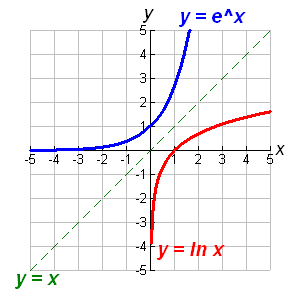
\includegraphics[scale=0.7]{images/003.png} \end{center}

\subsection{Position}
$\overrightarrow{OM}=r\sin(\theta)\cos(\phi)\overrightarrow{i}+r\sin(\theta)\sin(\phi)\overrightarrow{j}+r\cos(\theta)\overrightarrow{k}$

\newpage

\section{Les forces}
\subsection{Première loi de Newton}
<<Tout corps persévère dans l’état de repos ou de mouvement uniforme en ligne droite dans lequel il se trouve, à moins qu’une force n’agisse sur lui et ne le contraigne à changer d’état.>>
$$\overrightarrow{v}=C^{ste}\Rightarrow \sum\overrightarrow{F}=\overrightarrow{0}$$

\subsection{Deuxième loi de Newton}
<<Les changements qui arrivent dans le mouvement sont proportionnels à la force motrice et se font dans la ligne droite dans laquelle cette force a été imprimée.>>
$$\diff{}{t}(m\overrightarrow{V})=\overrightarrow{F}$$
$$\int_{t_1}^{t_2}\overrightarrow{F}(t)dt=m\overrightarrow{V_{t_2}}-m\overrightarrow{V_{t_1}}\text{\textit{ si m est constante}}$$

\subsection{Troisième loi de Newton}
<<L'action est toujours égale et opposée à la réaction, c'est-à-dire que les actions de deux corps l'un sur l'autre sont toujours égales et dans des directions contraires.>>
$$\overrightarrow{F}_{a/b}=-\overrightarrow{F}_{b/a}$$

\subsection{Types de force}
Il existe deux types de forces : les forces fondamentales (gravitation, électrique, forte et faible) et les forces phénoménologiques (frottements,...).\\\\\\


Les "forces de réaction": chaque corps exerce une force sur un autre corps qui est en contact avec lui. Par exemple, si un objet repose sur une table, cette table exerce une force égale et opposée sur l'objet. Cette force est toujours normale au support.\\

Les "forces de frottement": la force de frottement existe lorsque deux corps sont en contact. Elle s'oppose toujours au mouvement. La force de frottement qui s'oppose au mouvement n'a pas seulement un effet négatif, elle est indispensable pour assurer aussi le contact entre deux surfaces.\\

Les "forces de tension" exercées sur un corps: c'est une force qui tire sur un élément d'un corps comme par exemple, la tension exercée par un fil, par un ressort.\\

Les "forces à distance": ce sont les forces qui agissent par l'intermédiaire de champs vectoriels comme par exemple le champ électrique, le champ magnétique, le champ gravitationnel. Ce dernier a comme particularité s'il est isotrope de pouvoir se réduire à l'étude du centre de gravité du corps.


\newpage

\section{Notions diverses}
\subsection{Quantité de mouvement}
La quantité de mouvement d'un corps de masse $m$ est $\overrightarrow{p}=m\overrightarrow{v}$.

\subsection{Conservation de la quantité de mouvement}
Soit un système isolé dans un référentiel Galiléen, d'après la troisième loi de Newton pour chaque force appliquée d'un corps a sur un corps b il existe une force de même valeur et de sens inverse appliquée par b sur a.\\

Ainsi en faisant la somme des forces appliquées sur chacun des corps i du système isolé, on obtient $\sum\overrightarrow{F}=\sum m_ia_i=\overrightarrow{0}$.\\

Donc en intégrant (la masse totale est constante), on obtient $\sum m_iv_i=C^{ste}$. Ainsi la quantité de mouvement du système isolé dans un référentiel Galiléen se conserve.

\subsection{Centre de masse}
Le centre de masse d'un ensemble de corps i dans un système isolé est $\displaystyle \overrightarrow{C_m}=\frac{\sum m_i \overrightarrow{OM}_i}{\sum m_i}$.


% ------------------------------------------------------------------------------------------------------ %
% ------------------------------------------------------------------------------------------------------ %



% ------------------------------------------------------------------------------------------------------ %
% ------------------------------------------------------------------------------------------------------ %


\chapter{Changement de référentiel}
\section*{Produit vectoriel}
\subsection*{Définition}
Le produit vectoriel $\vec{w}=\vec{u}\wedge\vec{v}$ de deux vecteurs $\vec{u}(u_1,u_2,u_3)$ et $\vec{v}(v_1,v_2,v_3)$ est un vecteur $\vec{w}$ orthonormal à $\vec{u}$ et à $\vec{v}$ tel que $||\vec{w}||=||\vec{u}\wedge\vec{v}||=||\vec{u}||\cdot ||\vec{v}||\cdot \sin((\vec{u},\vec{v}))$.\\

On a $\begin{pmatrix}
u_1 \\ u_2 \\ u_3
\end{pmatrix}\wedge \begin{pmatrix}
v_1 \\ v_2 \\ v_3
\end{pmatrix}=\begin{pmatrix}
u_2v_3-u_3v_2 \\
u_3v_1-u_1v_3 \\
u_1v_2-u_2v_1
\end{pmatrix}$.\\\\

$\vec{u}\wedge\vec{u}=0$ et plus généralement si $\vec{u}$ et $\vec{v}$ sont colinéaires, $\vec{u}\wedge\vec{v}=\vec{0}$.

\subsection*{Dérivation}
Soient $\vec{u}\begin{pmatrix}
u_1 \\ u_2 \\ u_3
\end{pmatrix}$ et $\vec{v}\begin{pmatrix}
v_1 \\ v_2 \\ v_3
\end{pmatrix}$, alors $\vec{u}'\begin{pmatrix}
u_1' \\ u_2' \\ u_3'
\end{pmatrix}$ et $\vec{v}'\begin{pmatrix}
v_1' \\ v_2' \\ v_3'
\end{pmatrix}$.\\\\

$\begin{array}{rcl}
\text{On a donc }(\vec{u}\wedge\vec{v})'&=&\begin{pmatrix}
u_2v_3-u_3v_2 \\
u_3v_1-u_1v_3 \\
u_1v_2-u_2v_1
\end{pmatrix}'=\begin{pmatrix}
u_2'v_3+u_2v_3'-u_3'v_2-u_3v_2' \\
u_3'v_1+u_3v_1'-u_1'v_3-u_1v_3' \\
u_1'v_2+u_1v_1'-u_2'v_1-u_2v_1'
\end{pmatrix}\\\\
&=&\begin{pmatrix}
u_2'v_3-u_3'v_2 \\
u_3'v_1-u_1'v_3 \\
u_1'v_2-u_2'v_1
\end{pmatrix}+\begin{pmatrix}
u_2v_3'-u_3v_2'\\
u_3v_1'-u_1v_3'\\
u_1v_1'-u_2v_1'
\end{pmatrix}=\vec{u}'\wedge\vec{v}+\vec{u}\wedge\vec{v}'
\end{array}$

\section{Mouvement relatif des référentiels}
Soient un point $M$ et deux référentiels $\mathcal{R}_a(0,\overrightarrow{e}_x,\overrightarrow{e}_y,\overrightarrow{e}_z)$ et $\mathcal{R}_e(0,\overrightarrow{e}_{x_1},\overrightarrow{e}_{y_1},\overrightarrow{e}_{z_1})$.\\

Si l'on connaît la trajectoire de $\overrightarrow{OM}_{\mathcal{R}_a}$, ainsi que la vitesse $\overrightarrow{v}_{M/\mathcal{R}_a}$ et l'accélération $\overrightarrow{a}_{M/\mathcal{R}_a}$ du point $M$ dans $\mathcal{R}_a$, quelles sont la trajectoire $OM_{\mathcal{R}_e}$, la vitesse $\overrightarrow{v}_{M/\mathcal{R}_e}$ et l'accélération $\overrightarrow{a}_{M/\mathcal{R}_e}$ du point $M$ dans $\mathcal{R}_e$ ?

\subsection{Mouvement d’entraînement, référentiel fixe et absolu}
Le mouvement de $\mathcal{R}_e$ par rapport à $\mathcal{R}_a$ est appelé le mouvement d’entraînement.\\\\
Le référentiel que l'on considère comme immobile  ($\mathcal{R}_a$) est appelé le référentiel fixe ou absolu.\\ L'autre référentiel ($\mathcal{R}_e$) est appelé référentiel mobile ou référentiel relatif.

\newpage

\subsection{Rotation relative des repères}
\subsubsection{Vecteur rotation d'entraînement}
Il existe un vecteur nommé vecteur rotation d'entraînement de $\mathcal{R}_e$ par rapport à\\
$\mathcal{R}_a$ noté $\overrightarrow{\Omega}_{\mathcal{R}_e/\mathcal{R}_a}$ tel que :
$$\left\{\begin{array}{rcl} \diff*{\overrightarrow{e}_{x_1}}{t}{\mathcal{R}_a}=\overrightarrow{\Omega}_{\mathcal{R}_e/\mathcal{R}_a}\times\overrightarrow{e_{x_1}}\\\\
\diff*{\overrightarrow{e}_{y_1}}{t}{\mathcal{R}_a}=\overrightarrow{\Omega}_{\mathcal{R}_e/\mathcal{R}_a}\times\overrightarrow{e_{y_1}}\\\\
\diff*{\overrightarrow{e}_{z_1}}{t}{\mathcal{R}_a}=\overrightarrow{\Omega}_{\mathcal{R}_e/\mathcal{R}_a}\times\overrightarrow{e_{z_1}}
\end{array}\right.$$

\subsection{Translation et rotation}
Le mouvement d’entraînement de $\mathcal{R}_e$ par rapport à $\mathcal{R}_a$ est la superposition :
\begin{itemize}[label=$\bullet$]
\item d'une rotation à la vitesse angulaire $\overrightarrow{\Omega}_{\mathcal{R}_e/\mathcal{R}_a}$
\item d'une translation caractérisée par $\overrightarrow{v}_{O_e/\mathcal{R}_a}=\diff*{\overrightarrow{O_aO_e}}{t}{\mathcal{R}_a}$
\end{itemize}

Avec $O_{e}$ un point fixe dans $\mathcal{R}_e$ et $O_{\mathcal{R}_a}$ un point fixe dans $\mathcal{R}_a$.

\begin{center}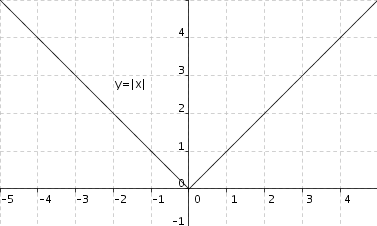
\includegraphics[scale=0.4]{images/004.png}\end{center}

\subsection{Mouvement d’entraînement par translation}
On a \phantom{aaa}$\left\{ \begin{array}{rcl}
\diff*{\overrightarrow{e}_{x_1}}{t}{\mathcal{R}_a}=\overrightarrow{\Omega}_{\mathcal{R}_e/\mathcal{R}_a}\times\overrightarrow{e_{x_1}}=\vec{0}\\
\diff*{\overrightarrow{e}_{y_1}}{t}{\mathcal{R}_a}=\overrightarrow{\Omega}_{\mathcal{R}_e/\mathcal{R}_a}\times\overrightarrow{e_{y_1}}=\vec{0}\\
\diff*{\overrightarrow{e}_{z_1}}{t}{\mathcal{R}_a}=\overrightarrow{\Omega}_{\mathcal{R}_e/\mathcal{R}_a}\times\overrightarrow{e_{z_1}}=\vec{0}
\end{array}  \right. \Leftrightarrow \overrightarrow{\Omega}_{\mathcal{R}_e/\mathcal{R}_a}=\vec{0}$

\begin{center}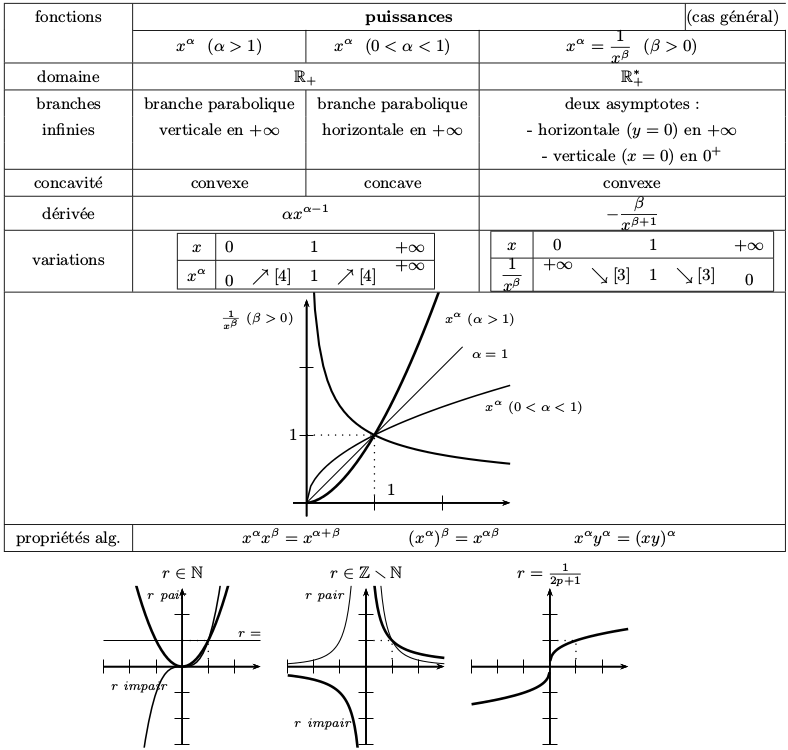
\includegraphics[scale=0.25]{images/005.png}\end{center}

\newpage

\subsection{Mouvement d’entraînement par rotation}
Si $(O_{z_a})=(O_{z_{e}})$ et $O_a=O_e$, le référentiel $\mathcal{R}_e$ est en rotation dans le référentiel $\mathcal{R}_a$ autour de la verticale, alors 
\begin{center}$\left\{\begin{array}{rcl} 
\overrightarrow{e_{x_e}} &=&\cos(\theta)\overrightarrow{e_{x_a}} +\sin(\theta)\overrightarrow{e_{y_a}}\\
\overrightarrow{e_{y_e}} &=&-\sin(\theta)\overrightarrow{e_{x_a}} +\cos(\theta)\overrightarrow{e_{y_a}}\\
\overrightarrow{e_{z_e}} &=&\overrightarrow{e_{z_a}}
\end{array}\right.$\end{center}

et donc 
\begin{center}$\left\{\begin{array}{rcl}
\diff*{\overrightarrow{e_{x_e}}}{t}{\mathcal{R}_a}&=&\dot{\theta}(-\sin(\theta)\overrightarrow{e_{x_a}} +\cos(\theta)\overrightarrow{e_{y_a}})=\dot{\theta}\overrightarrow{e_{y_e}}\\
\diff*{\overrightarrow{e_{y_e}}}{t}{\mathcal{R}_a}&=&\dot{\theta}(-\cos(\theta)\overrightarrow{e_{x_a}} -\sin(\theta)\overrightarrow{e_{y_a}})=-\dot{\theta}\overrightarrow{e_{x_e}}\\
\diff*{\overrightarrow{e_{z_e}}}{t}{\mathcal{R}_a}&=&\overrightarrow{0}
\end{array}\right.$\end{center}

\bigskip

Or on a
\begin{center}$\left\{\begin{array}{rcccl}
\dot{\theta}\overrightarrow{e_{z_e}}\times \overrightarrow{e_{x_e}} &=&\dot{\theta}\overrightarrow{e_{y_e}} &=&\diff*{\overrightarrow{e_{x_e}}}{t}{\mathcal{R}_a}\\
\dot{\theta}\overrightarrow{e_{z_e}}\times \overrightarrow{e_{y_e}} &=&-\dot{\theta}\overrightarrow{e_{x_e}} &=&\diff*{\overrightarrow{e_{y_e}}}{t}{\mathcal{R}_a}\\
\dot{\theta}\overrightarrow{e_{z_e}}\times \overrightarrow{e_{z_e}} &=&\overrightarrow{0} &=&\diff*{\overrightarrow{e_{x_e}}}{t}{\mathcal{R}_a}
\end{array}\right.$\end{center}

\bigskip

Donc en posant $\overrightarrow{\Omega}=\dot{\theta}\overrightarrow{e_{z_a}}$, pour $i=x$, $y$ ou $z$ :
$\diff*{\overrightarrow{e_{i_e}}}{t}{}=\overrightarrow{\Omega}\times \overrightarrow{e_{i_e}}$.

\bigskip

Alors $\overrightarrow{\Omega}$ représente le vecteur rotation de $\mathcal{R}_e$ par rapport à $\mathcal{R}_a$:
$$\overrightarrow{\Omega}_{\mathcal{R}_e/\mathcal{R}_a}=\overrightarrow{\Omega}=\dot{\theta}\overrightarrow{e_{z_a}}$$

\bigskip

\begin{center}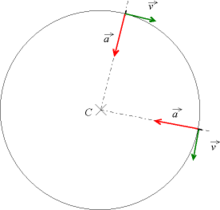
\includegraphics[scale=0.5]{images/006.png}\end{center}

\newpage

\section{Dérivation d'un vecteur par rapport au temps}
\subsection{Formule de Varignon}
Soit un vecteur quelconque $\overrightarrow{U}$, on peut le projeter dans $\mathcal{R}_e$ : $$\overrightarrow{U}=U_{x_e}\overrightarrow{e_{x_e}}+U_{y_e}\overrightarrow{e_{y_e}}+ U_{z_e}\overrightarrow{e_{z_e}}$$\\
On peut dériver ce vecteur par rapport au temps dans le référentiels $\mathcal{R}_a$ :\\
$$\begin{array}{rcl}\diff*{\overrightarrow{U}}{t}{\mathcal{R}_a}&=&\dot{U}_{x_e}\overrightarrow{e_{x_e}} +\dot{U}_{y_e}\overrightarrow{e_{y_e}} +\dot{U}_{z_e}\overrightarrow{e_{z_e}} +U_{x_e}\diff*{\overrightarrow{e_{x_e}}}{t}{\mathcal{R}_a} +U_{y_e}\diff*{\overrightarrow{e_{y_e}}}{t}{\mathcal{R}_a} +U_{z_e}\diff*{\overrightarrow{e_{x_e}}}{t}{\mathcal{R}_a}\\
&=&\diff*{\overrightarrow{U}}{t}{\mathcal{R}_e}+\overrightarrow{\Omega}_{\mathcal{R}_e/\mathcal{R}_a}\times (U_{x_e}\overrightarrow{e}_{x_e} +U_{y_e}\overrightarrow{e}_{y_e} +U_{z_e}\overrightarrow{e}_{z_e})\end{array}$$\\\\
$$\Leftrightarrow\diff*{\overrightarrow{U}}{t}{\mathcal{R}_a}=\diff*{\overrightarrow{U}}{t}{\mathcal{R}_e}+\overrightarrow{\Omega}_{\mathcal{R}_e/\mathcal{R}_a}\times \overrightarrow{U}$$\\

\section{Composition des vitesses}
\subsection{Vitesse absolue et vitesse relative}
Pour un point M quelconque, on cherche la relation entre sa vitesse absolue $\overrightarrow{v_{M/\mathcal{R}_a}}$ définie dans le référentiel absolu $\mathcal{R}_a$ et sa vitesse relative $\overrightarrow{v_{M/\mathcal{R}_e}}$ définie dans le référentiel relatif $\mathcal{R}_e$. \\\\

On a $\overrightarrow{v_{M/\mathcal{R}_a}}=\diff*{\overrightarrow{O_aM}}{t}{\mathcal{R}_a}=\overrightarrow{v_a}$ et $\overrightarrow{v_{M/\mathcal{R}_e}}=\diff*{\overrightarrow{O_eM}}{t}{\mathcal{R}_e}=\overrightarrow{v_e}$.\\\\\\

Comme $\overrightarrow{O_aM}=\overrightarrow{O_aO_e}+\overrightarrow{O_eM}$, on a :
$$\begin{array}{rcl}\overrightarrow{v_{M/\mathcal{R}_a}}=\diff*{\overrightarrow{O_aM}}{t}{\mathcal{R}_a}
&=&\diff*{\overrightarrow{O_aO_e}}{t}{\mathcal{R}_a}+ \diff*{\overrightarrow{O_eM}}{t}{\mathcal{R}_a}\\\\
&=&\overrightarrow{v_{O_e/\mathcal{R}_a}}+\diff*{\overrightarrow{O_eM}}{t}{\mathcal{R}_e}+\overrightarrow{\Omega}_{\mathcal{R}_e/\mathcal{R}_a}\times \overrightarrow{O_eM}\end{array}$$

\subsubsection{Loi de composition des vitesses}
On en déduit la loi de composition des vitesses $$\overrightarrow{v_{M/\mathcal{R}_a}}=\overrightarrow{v_{O_e/\mathcal{R}_a}}+\overrightarrow{v_{M/\mathcal{R}_e}}+\overrightarrow{\Omega}_{\mathcal{R}_e/\mathcal{R}_a}\times \overrightarrow{O_eM}$$

\newpage

\subsection{Point coïncidant}
\subsubsection{Définition}
Le point coïncidant noté $M^*$ est le point :\begin{itemize}[label=$\bullet$]
\item fixe dans $\mathcal{R}_e$
\item qui coïncide avec M
\item à l'instant t considéré
\end{itemize}

\subsubsection{Remarque}
Le point coïncidant est un point géométrique puisqu'il est fixe dans $\mathcal{R}_e$ et non un point matériel comme le point M.

\subsubsection{Conséquence}
La fixité du point $M^*$ dans $\mathcal{R}_e$ implique que $\overrightarrow{v_{M^*/\mathcal{R}_e}} =\overrightarrow{0}$
et donc la loi de composition des vitesses appliquée au point $M^*$ donne :\\
$$\overrightarrow{v_{M^*/\mathcal{R}_a}}=\overrightarrow{v_{O_e/\mathcal{R}_a}}+\cancel{\overrightarrow{v_{M^*/\mathcal{R}_e}}}+\overrightarrow{\Omega}_{\mathcal{R}_e/\mathcal{R}_a}\times \overrightarrow{O_eM^*} =\overrightarrow{v_e}(M)$$ avec $M^*(t)=M(t)$.

\subsection{Vitesse d'entraînement}
\subsubsection{Définition}
On appelle vitesse d’entraînement du point M, notée $\overrightarrow{v_e}(M)$, la vitesse qu'aurait le point M dans le référentiel absolu si M était fixe dans $\mathcal{R}_e$, c'est-à-dire si M était entraîné par le mouvement d'entraînement du référentiel relatif $\mathcal{R}_e$.

\subsubsection{Propriétés}
\begin{enumerate}
\item On constate que la vitesse d'entraînement du point M correspond à la vitesse absolue\\
du point coïncidant $M^*$ : $$\overrightarrow{v_e}(M)=
\overrightarrow{v_{M^*/\mathcal{R}_a}} =\overrightarrow{v_{O_e/\mathcal{R}_a}} +\overrightarrow{\Omega}_{\mathcal{R}_e/\mathcal{R}_a} \times \overrightarrow{O_eM}$$\\

\item La loi de composition des vitesses s'écrit alors :\\
$$\overrightarrow{v_a}=\overrightarrow{v_r}+\overrightarrow{v_e} \Leftrightarrow \underbrace{\overrightarrow{v_{M/\mathcal{R}_a}}}_{\text{vitesse absolue}}=\underbrace{\overrightarrow{v_{M/\mathcal{R}_e}}}_{\text{vitesse relative}}+\underbrace{\overrightarrow{v_e}(M)}_{\text{vitesse d'entraînement}}$$
\end{enumerate}

\newpage

\section{Composition des accélérations}
\subsection{Accélération absolue et accélération relative}
On a $\overrightarrow{a_{M/\mathcal{R}_a}}=\diff*{\overrightarrow{v_{M/\mathcal{R}_a}}}{t}{\mathcal{R}_a}$ donc on repart de la loi de composition des vitesses :
$$\overrightarrow{v_{M/\mathcal{R}_a}}= \overrightarrow{v_{M/\mathcal{R}_e}}+ \overrightarrow{v_{O_e/\mathcal{R}_a}}+\overrightarrow{\Omega}_{\mathcal{R}_e/\mathcal{R}_a}\times \overrightarrow{O_eM}$$
que l'on dérive par rapport au temps terme à terme :
$$\diff*{\overrightarrow{v_{M/\mathcal{R}_a}}}{t}{\mathcal{R}_a}=\diff*{\overrightarrow{v_{M/\mathcal{R}_e}}}{t}{\mathcal{R}_a}+ \diff*{\overrightarrow{v_{O_e/\mathcal{R}_a}}}{t}{\mathcal{R}_a}+ \diff*{(\overrightarrow{\Omega}_{\mathcal{R}_e/\mathcal{R}_a}\times \overrightarrow{O_eM})}{t}{\mathcal{R}_a}$$\\

En introduisant la notation simplifiée $\overrightarrow{\Omega} =\overrightarrow{\Omega}_{\mathcal{R}_e/\mathcal{R}_a}$, ces dérivées deviennent :

$$\begin{array}{rcl}
\diff*{\overrightarrow{v_{M/\mathcal{R}_e}}}{t}{\mathcal{R}_e}&=&\diff*{\overrightarrow{v_{M/\mathcal{R}_e}}}{t}{\mathcal{R}_a}+\overrightarrow{\Omega}\times \overrightarrow{v_{M/\mathcal{R}_e}}= \overrightarrow{a_{M/\mathcal{R}_e}}+ \overrightarrow{\Omega}\overrightarrow{v_{M/\mathcal{R}_e}}\\\\
\diff*{\overrightarrow{v_{O_e/\mathcal{R}_a}}}{t}{\mathcal{R}_a}&=&\overrightarrow{a_{O_e/\mathcal{R}_a}}\\\\\\
\diff*{(\overrightarrow{\Omega}_{\mathcal{R}_e/\mathcal{R}_a}\times \overrightarrow{O_eM})}{t}{\mathcal{R}_a}&=&
\diff{\overrightarrow{\Omega}}{t}\times\overrightarrow{O_eM}+\overrightarrow{\Omega}\times \diff*{\overrightarrow{O_eM}}{t}{\mathcal{R}_a}\\\\
&=&\diff{\overrightarrow{\Omega}}{t}\times\overrightarrow{O_eM}+\overrightarrow{\Omega}\times \left[\diff*{\overrightarrow{O_eM}}{t}{\mathcal{R}_e}+\overrightarrow{\Omega}\times \overrightarrow{O_eM}\right]\\\\
&=&\overrightarrow{\Omega}\times (\overrightarrow{\Omega}\times \overrightarrow{O_eM})+\diff{\overrightarrow{\Omega}}{t}\times \overrightarrow{O_eM}+\overrightarrow{\Omega}\times \overrightarrow{v_{M/\mathcal{R}_e}}\end{array}$$

\subsubsection{Loi de composition des accélérations}
On en déduit la loi de composition des accélérations :

$$\overrightarrow{a_{M/\mathcal{R}_a}}=\overrightarrow{a_{M/\mathcal{R}_e}}+\overrightarrow{a_{O_e/\mathcal{R}_a}}+\overrightarrow{\Omega}\times (\overrightarrow{\Omega}\times \overrightarrow{O_eM})+\diff{\overrightarrow{\Omega}}{t}\times \overrightarrow{O_eM}+2\overrightarrow{\Omega}\times \overrightarrow{v_{M/\mathcal{R}_e}}$$

avec $\overrightarrow{a_{M/\mathcal{R}_a}}$ l'accélération absolue et $\overrightarrow{a_{M/\mathcal{R}_e}}$ l'accélération relative.

\newpage

\subsection{Point coïncidant}
\subsubsection{Loi de composition des accélérations}
Par définition du point coïncidant il s'agit d'un point fixe du référentiel relatif, on a donc : \\
$\overrightarrow{v_{M^*/\mathcal{R}_e}}=\overrightarrow{0}$ et $\overrightarrow{a_{M^*/\mathcal{R}_e}}=\overrightarrow{0}$.\\

On obtient, avec $M^*(t)=M(t)$ :
$$\begin{array}{rcl}\overrightarrow{a_{M^*/\mathcal{R}_a}}&=&\cancel{\overrightarrow{a_{M^*/\mathcal{R}_e}}}+\overrightarrow{a_{O_e/\mathcal{R}_a}}+ \overrightarrow{\Omega}\times (\overrightarrow{\Omega}\times \overrightarrow{O_eM^*})+\diff{\overrightarrow{\Omega}}{t}\times \overrightarrow{O_eM^*} +2\overrightarrow{\Omega}\times \cancel{\overrightarrow{v_{M^*/\mathcal{R}_e}}}\\
&=&\overrightarrow{a_{O_e/\mathcal{R}_a}}+ \overrightarrow{\Omega}\times (\overrightarrow{\Omega}\times \overrightarrow{O_eM^*})+\diff{\overrightarrow{\Omega}}{t}\times \overrightarrow{O_eM^*}\end{array}$$

\subsection{Accélération d'entraînement}
\subsubsection{Définition}
On appelle accélération d’entraînement du point M, notée $\overrightarrow{a_e}(M)$,
l'accélération qu'aurait le point M dans le référentiel absolu si M était fixe dans $\mathcal{R}_e$, c'est-à-dire si M était entraîné par le mouvement d'entraînement du référentiel relatif de $\mathcal{R}_e$.

\subsubsection{Propriété}
L'accélération d'entraînement de M est l'accélération absolue du point coïncidant $M^*$ :
$$\overrightarrow{a_e}(M)=\left\{ \begin{array}{lll}
\overrightarrow{a_{M^*/\mathcal{R}_a}}\\
\overrightarrow{a_{O_e/\mathcal{R}_a}}+\overrightarrow{\Omega}\times (\overrightarrow{\Omega}\times \overrightarrow{O_eM})+\diff{\overrightarrow{\Omega}}{t}\times \overrightarrow{O_eM}
\end{array}\right.$$\\

\subsection{Accélération d'entraînement de Coriolis}
D'après la définition de l'accélération relative et de l'accélération d'entraînement, la loi de composition des accélérations s'écrit :
$$\overrightarrow{a_{M/\mathcal{R}_a}}=\overrightarrow{a_{M/\mathcal{R}_e}}+\overrightarrow{a_e}(M)+2\overrightarrow{\Omega}\times \overrightarrow{v_{M/\mathcal{R}_e}}$$

\subsubsection{Définition}
On appelle accélération de Coriolis, notée $\overrightarrow{a_C}(M)$, le terme :
$$\overrightarrow{a_C}(M)=2\overrightarrow{\Omega}_{\mathcal{R}_e/\mathcal{R}_a}\times \overrightarrow{v_{M/\mathcal{R}_e}}\Leftrightarrow\overrightarrow{a_C}(M)=2\Omega\times \overrightarrow{v_r}$$

\subsection{Accélération d'entraînement}
La loi de composition des accélérations s'écrit donc :
$$\overrightarrow{a_a}=\overrightarrow{a_r}+\overrightarrow{a_e}+\overrightarrow{a_C}\Leftrightarrow \underbrace{\overrightarrow{a_{M/\mathcal{R}_a}}}_{\text{accél. absolue}}=\underbrace{\overrightarrow{a_{M/\mathcal{R}_e}}}_{\text{accél. relative}}+ \underbrace{\overrightarrow{a_e}(M)}_{\text{accél. d'entraînement}} +\underbrace{\overrightarrow{a_C}(M)}_{\text{accél. de Coriolis}}$$


% ------------------------------------------------------------------------------------------------------ %
% ------------------------------------------------------------------------------------------------------ %



% ------------------------------------------------------------------------------------------------------ %
% ------------------------------------------------------------------------------------------------------ %


\chapter{Dynamique dans un référentiel non Galiléen}
\section{Définitions}
\subsection{Définition de principe}
Un référentiel galiléen est un référentiel dans lequel un point matériel isolé a un mouvement rectiligne uniforme :
$$m\overrightarrow{a_M/\mathcal{R}}=\overrightarrow{F}=\overrightarrow{0}$$

\subsection{Définition pratique}
\`{A} partir de la deuxième loi de Newton, un référentiel est galiléen si et seulement si l'on peut appliquer le principe fondamental de la dynamique sur un point $M$ de masse $m$, donc si l'on a :
$$m\overrightarrow{a_M/\mathcal{R}_g}=\overrightarrow{F}$$

\section{Propriétés des référentiels Galiléens}
Soit $M$ pseudo-isolé, supposons qu'on l'étudie dans deux référentiels galiléens $\mathcal{R}_g$ et $\mathcal{R}'_g$ : on a donc $m\overrightarrow{a_M/\mathcal{R}_g}=\overrightarrow{0}$ et $m\overrightarrow{a_M/\mathcal{R}'_g}=\overrightarrow{0}$.\\

On sait que 
$$\overrightarrow{a_M/\mathcal{R}_g}=\overrightarrow{a_M/\mathcal{R}'_g}+\overrightarrow{a_e}(M)+2\overrightarrow{\Omega}_{\mathcal{R}'_g/\mathcal{R}_g}\times \overrightarrow{v_{M/\mathcal{R}'_g}}$$\\
d'où pour tout point $M$ pseudo-isolé :\\ $$\overrightarrow{a_e}(M)+2\overrightarrow{\Omega}_{\mathcal{R}'_g/\mathcal{R}_g}\times \overrightarrow{v_{M/\mathcal{R}'_g}}=\overrightarrow{0}
\Leftrightarrow \left\{\begin{array}{rcl} \overrightarrow{\Omega}_{\mathcal{R}'_g/\mathcal{R}_g}&=&\overrightarrow{0} \\
\overrightarrow{a_e}(M)&=&\overrightarrow{0} \end{array}\right.$$

$\overrightarrow{\Omega}_{\mathcal{R}'_g/\mathcal{R}_g}=\overrightarrow{0}$ : $\mathcal{R}_g$ et $\mathcal{R}'_g$ sont en translation l'un par rapport à l'autre

$\overrightarrow{a_e}(M)=\overrightarrow{0}$ : cette translation est rectiligne uniforme


\subsubsection{Relation entre les référentiels Galiléens}
Tous les référentiels Galiléens sont en translation rectiligne uniforme les uns par rapport aux autres ; et donc par rapport à l’un d’entre eux.\\

Ainsi si un référentiel Galiléen est connu, tous les autres s’en déduisent par translations rectilignes uniformes.


\section{Dynamique dans un référentiel non Galiléen}
\subsection{Principe fondamental de la dynamique}
Dans un référentiel Galiléen $\mathcal{R}_g$, le principe fondamental de la dynamique pour un objet M de masse m s'écrit $m\overrightarrow{a_{M/\mathcal{R}_g}}=\overrightarrow{F}$.\\

Soit $\mathcal{R}$ un référentiel non Galiléen, il possède un mouvement d'entraînement par rapport à $\mathcal{R}_g$ qui conduit à la loi de composition des accélérations : $\overrightarrow{a_a}=\overrightarrow{a_r}+\overrightarrow{a_e}+\overrightarrow{a_C}$, c'est-à-dire :
$$\overrightarrow{a_{M/\mathcal{R}_g}}=\overrightarrow{a_{M/\mathcal{R}}}+\overrightarrow{a_e}(M)+\overrightarrow{a_C}(M)$$\\
Dès lors, le principe fondamental de la dynamique dans $\mathcal{R}_g$ peut s'écrire sous la forme :
$$m\overrightarrow{a_{M/\mathcal{R}_g}}=\overrightarrow{F} \Leftrightarrow m\overrightarrow{a_{M/\mathcal{R}}}+m\overrightarrow{a_e}(M)+m\overrightarrow{a_C}(M)=\overrightarrow{F}$$\\
On peut donc étudier le mouvement de $M$ dans $\mathcal{R}$ et lui associer une relation fondamentale de la dynamique adaptée à la nature non galiléenne de $\mathcal{R}$ en écrivant
$m\overrightarrow{a_{M/\mathcal{R}}}=\overrightarrow{F}-m\overrightarrow{a_e}(M)-m\overrightarrow{a_C}(M)$.

\subsection{Pseudo-forces}
On appelle pseudo-forces ou forces d'inertie deux termes homogènes à une "vraie" force :
\begin{itemize}
\item la force d'inertie d'entraînement : $\overrightarrow{F_{ie}}=-m\cdot\overrightarrow{a_e}(M)$.
\item la force d'inertie de Coriolis : $\overrightarrow{F_C}=-m\cdot \overrightarrow{a_C}(M)$.
\end{itemize}

\bigskip

On applique le principe fondamental de la dynamique à un point matériel M de masse m, étudié dans un référentiel $\mathcal{R}$ non galiléen (relativement à un référentiel galiléen $\mathcal{R}_g$) :
$$m\cdot \overrightarrow{a_{M/\mathcal{R}}}=\overrightarrow{F}+ \overrightarrow{F_{ie}}+\overrightarrow{F_C}
\text{ avec : } 
\left\{\begin{array}{rcll}
\overrightarrow{F}&=&\sum\limits_i \overrightarrow{F}_{i\rightarrow M}&\text{ la résultante des "vraies" forces}\\
\overrightarrow{F_{ie}}&=&-m\cdot \overrightarrow{a_e}(M)&\text{ la force d'inertie d'entraînement}\\
\overrightarrow{F_{C}}&=&-m\cdot \overrightarrow{a_C}(M)&\text{ la force d'inertie de Coriolis}
\end{array}\right.$$

\subsection{Méthodes}
\begin{enumerate}
\item Comment exprime-t-on la force d'inertie d'entraînement ?\\

L'accélération d'inertie d'entraînement est l'accélération du point coïncidant, donc :
$$\overrightarrow{F_{ie}}=-m\cdot\overrightarrow{a_e}(M)=-m\cdot \overrightarrow{a_{M^*/\mathcal{R}_g}}$$
où $M^*$ est le point coïncidant associé à $M$ étudié dans $\mathcal{R}$, c'est-à-dire 
le point qui est fixe dans $\mathcal{R}$ le référentiel relatif  et qui coïncide avec $M$ à l'instant $t$.\\

\item Comment exprime-t-on la force d’inertie de Coriolis ?\\

L'accélération d'inertie de Coriolis est :
$$\overrightarrow{F_C}=-m\cdot \overrightarrow{a_C}(M)=-2m\cdot \overrightarrow{\Omega}_{\mathcal{R}/\mathcal{R}_g}\times \overrightarrow{v_{M/\mathcal{R}}}$$
où $\overrightarrow{\Omega}_{\mathcal{R}/\mathcal{R}_g}$ est le vecteur rotation du référentiel relatif $\mathcal{R}$ par rapport au référentiel galiléen $\mathcal{R}_g$ et $\overrightarrow{v_{M/\mathcal{R}}}$ est la vitesse du point $M$ dans le référentiel relatif.
\end{enumerate}


% ------------------------------------------------------------------------------------------------------ %
% ------------------------------------------------------------------------------------------------------ %



% ------------------------------------------------------------------------------------------------------ %
% ------------------------------------------------------------------------------------------------------ %


\chapter{Moment cinétique d'un point matériel}
\section{Définitions}
\subsection{Moment d'une force par rapport à un point}
Le moment évalué en un point $O$ de la force $\overrightarrow{F}$ exercée en $M$ est $\overrightarrow{\mathcal{M}_O}(\overrightarrow{F})=\overrightarrow{OM}\times \overrightarrow{F}$.\\\\

\subsection{Moment d'une force par rapport à un axe}
Soit $(\Delta)$ un axe passant par $O$ orienté selon son vecteur unitaire $\overrightarrow{e_{\Delta}}$.

On appelle moment de la force $\overrightarrow{F}$ par rapport à l'axe orienté $\Delta$ la projection scalaire\\
de $\overrightarrow{\mathcal{M}_O}(\overrightarrow{F})$ selon $\overrightarrow{e_\Delta}$ : $\mathcal{M}_{\Delta}=\overrightarrow{\mathcal{M}_O}(\overrightarrow{F})\cdot \overrightarrow{e_\Delta}$.\\\\

\subsection{Moment cinétique d'un point matériel}
Dans le référentiel $\mathcal{R}$, le moment cinétique du point matériel M de masse m en un point $O$ est :
$$\overrightarrow{L_{O/\mathcal{R}}}(M)=\overrightarrow{OM}\times \overrightarrow{p_{M/\mathcal{R}}} =\overrightarrow{OM}\times m\overrightarrow{v_{M/\mathcal{R}}}$$\\

\subsection{Moment cinétique par rapport à un axe}
Soit $(\Delta)$ un axe passant par $O$ orienté selon son vecteur unitaire $\overrightarrow{e_{\Delta}}$.\\

On appelle moment cinétique de $M$ par rapport à l'axe orienté $\Delta$ la projection scalaire de $\overrightarrow{L_{O/\mathcal{R}}}(M)$ selon $\overrightarrow{e_\Delta}$ : $L_\Delta = \overrightarrow{L_{O/\mathcal{R}}}\cdot \overrightarrow{e_\Delta}$.\\

Cette grandeur est indépendante du choix du point $O$, point quelconque de l'axe $\Delta$.

\newpage

\subsection{Interprétation physique}
Le moment cinétique est analogue à la quantité de mouvement :
\begin{itemize}
\item La quantité de mouvement est le produit de la vitesse par la masse qui mesure l'inertie d'un corps, c'est-à-dire la résistance qu'il oppose à toute modification de son état de mouvement.
\item Le moment cinétique est le produit de sa vitesse angulaire par une grandeur qui mesure son inertie de rotation, c'est-à-dire sa résistance à toute modification de son état de rotation.
\end{itemize}\bigskip

\subsection{Moment d'inertie}
\subsubsection{Définition}
On appelle moment d'inertie d'un corps, notée $J$, la grandeur qui mesure la résistance à toute modification de l'état de rotation de ce corps.\\

En général, le moment d'inertie $J=J_\Delta$ d'un objet dépend de l'axe $(\Delta)$ autour duquel on essaie de le faire tourner. Alors $L_\Delta=J_\Delta\cdot \omega$.\\

Le moment d’inertie d’un corps change si l’on modifie la façon dont sa masse est répartie autour de l’axe de rotation.

\begin{center}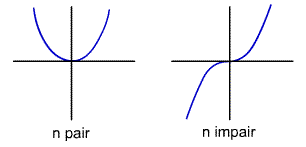
\includegraphics[scale=0.65]{images/008.png}\end{center}

\newpage

\begin{center}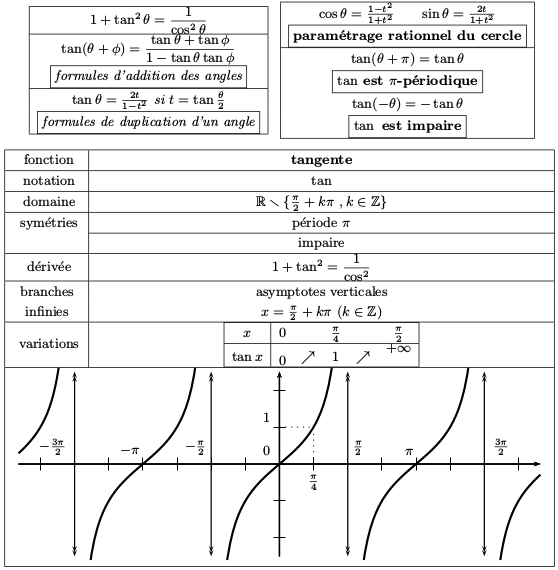
\includegraphics[scale=0.6]{images/009.png}\end{center}

\section{Moment cinétique dans un référentiel galiléen}
On choisit un point $O$ fixe de $\mathcal{R}$, donc tel que $\overrightarrow{v_{O/\mathcal{R}}}=\overrightarrow{0}$.\\
On dérive le moment cinétique de $M$ évalué en $O$ dans le référentiel galiléen $\mathcal{R}=\mathcal{R}_g$:
$$\begin{array}{rcl}
\diff*{\overrightarrow{L_{O/\mathcal{R}_g}(M)}}{t}{\mathcal{R}_g}= \diff{(\overrightarrow{OM}\times m\overrightarrow{v_{M/\mathcal{R}_g}})}{t} &=& \diff*{\overrightarrow{OM}}{t}{\mathcal{R}_g}\times m\overrightarrow{v_{M/\mathcal{R}_g}}+\overrightarrow{OM}\times m\diff*{\overrightarrow{v_{M/\mathcal{R}_g}}(M)}{t}{\mathcal{R}_g}\\\\
&=&\overrightarrow{v_{M/\mathcal{R}_g}}\times m\overrightarrow{v_{M/\mathcal{R}_g}}+\overrightarrow{OM}\times m\overrightarrow{a_{M/\mathcal{R}_g}}
\end{array}$$

\`{A} partir du principe fondamental de la dynamique, on obtient : $$m\overrightarrow{a_{M/\mathcal{R}_g}}=\overrightarrow{F_{ext}}$$

de plus $$\overrightarrow{OM}\times \overrightarrow{F_{ext}}=\overrightarrow{\mathcal{M}_O}(\overrightarrow{F_{ext}})$$
\bigskip

et donc 
$$\begin{array}{rcl}
\diff*{\overrightarrow{L_{O/\mathcal{R}_g}}(M)}{t}{\mathcal{R}_g}&=&\cancel{\overrightarrow{v_{M/\mathcal{R}_g}}\times m\overrightarrow{v_{M/\mathcal{R}_g}}}+\overrightarrow{OM}\times m\overrightarrow{a_{M/\mathcal{R}_g}}\\\\
&=&\overrightarrow{OM}\times \overrightarrow{F_{ext}}=\overrightarrow{\mathcal{M}_O}(\overrightarrow{F_{ext}})
\end{array}$$

\newpage

\subsubsection{Théorème du moment cinétique}
Pour un point matériel $M$ soumis à la résultante des forces $\overrightarrow{F_{ext}}$ dans un référentiel galiléen $\mathcal{R}_g$, observé depuis un point $O$ fixe dans $\mathcal{R}_g$ :\\
$$\diff*{\overrightarrow{L_{O/\mathcal{R}_g}}(M)}{t}{\mathcal{R}_g}=\overrightarrow{\mathcal{M}_O}(\overrightarrow{F_{ext}})\text{ avec }
\overrightarrow{L_{O/\mathcal{R}_g}}(M)=\overrightarrow{OM}\times m\overrightarrow{v_{M/\mathcal{R}_g}}\text{ et }
\overrightarrow{\mathcal{M}_O}(\overrightarrow{F_{ext}})=\overrightarrow{OM}\times\overrightarrow{F_{ext}}$$

\bigskip

\subsubsection{Théorème du moment cinétique selon un axe fixe $\Delta$ de $\mathcal{R}_g$}
Pour un point $M$ soumis à la résultante des forces $\overrightarrow{F_{ext}}$ dans un référentiel galiléen $\mathcal{R}_g$ :
$$\diff{L_\Delta}{t}=\mathcal{M}_\Delta\text{ avec }
\left\{\begin{array}{rcl}L_\Delta=\overrightarrow{L_{O/\mathcal{R}_g}}(M)\cdot \overrightarrow{e_\Delta}\\
\mathcal{M}_\Delta=\overrightarrow{\mathcal{M}_O}(\overrightarrow{F_{ext}})\cdot \overrightarrow{e_\Delta}\end{array}\right.$$\\

Si l'axe $\Delta$ est fixe dans $\mathcal{R}_g$ alors $$\overrightarrow{e_\Delta}=\overrightarrow{Cte}$$

donc $$\diff*{\overrightarrow{e_\Delta}}{t}{\mathcal{R}_g}=\overrightarrow{0}$$\\

On peut alors écrire $$\diff*{\overrightarrow{L_{O/\mathcal{R}_g}}(M)}{t}{\mathcal{R}_g}\cdot \overrightarrow{e_\Delta}=\left\{\begin{array}{rcl} \diff*{\overrightarrow{L_{O/\mathcal{R}_g}}(M)\cdot\overrightarrow{e_\Delta}}{t}{\mathcal{R}_g}&=& \diff{L_\Delta}{t}\\\\
\overrightarrow{\mathcal{M}_O}(\overrightarrow{F_{ext}})\cdot \overrightarrow{e_\Delta}&=&\mathcal{M}_\Delta
\end{array}\right.$$

\bigskip

\subsubsection{Conservation du moment cinétique}
$$\begin{array}{rcl}
\overrightarrow{L_{O/\mathcal{R}_g}}(M)=\overrightarrow{Cte}&\Leftrightarrow&\overrightarrow{\mathcal{M}_O}(\overrightarrow{F_{ext}}) =\overrightarrow{0}\\\\
&\Leftrightarrow&
\left\{ \begin{array}{rccl} \overrightarrow{F_{ext}}&=&\overrightarrow{0}&\text{ : }M\text{ est pseudo-isolé} \\
\overrightarrow{F_{ext}}&//&\overrightarrow{OM}&\text{ : }M\text{ est soumis à une force centrale} \end{array}\right.\end{array}$$

\newpage

\section{Forces centrales conservatives}
\subsection{Champ de forces centrales}
Soit $O$ un point fixe du référentiel $\mathcal{R}$ d'étude.\\
Lorsqu'en tout point $M$ de l'espace un point matériel est soumis à une force $\overrightarrow{F}(M)$ colinéaire au vecteur $\overrightarrow{OM}$, on parle de champ de forces centrales.\\

$\forall M\in \epsilon$, $\overrightarrow{OM}\times \overrightarrow{F}(M)=\overrightarrow{0} \Leftrightarrow \overrightarrow{F}$ est une force centrale\\

On appelle $O$ le centre de force. Avec la définition du vecteur unitaire $\overrightarrow{e_r}$ des coordonnées sphériques $\overrightarrow{e_r}=\frac{\overrightarrow{OM}}{OM}$, on peut écrire :
$\overrightarrow{F}(M)=F(M)\overrightarrow{e_r}$.\\

\begin{center}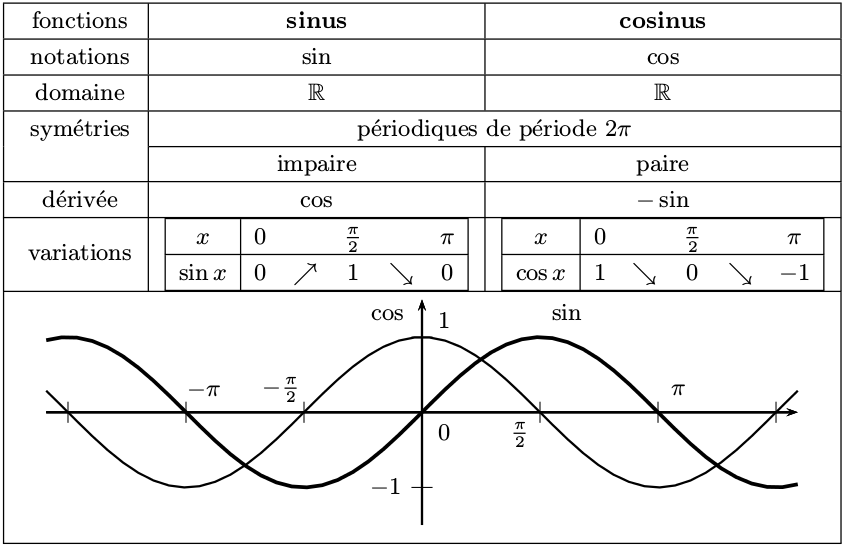
\includegraphics[scale=0.5]{images/010.png}\end{center}

\subsection{Champ de forces centrales conservatives}
Un champ de forces du type $\overrightarrow{F}(M)=F(r)\overrightarrow{e_r}$, avec $r=OM$ et $\overrightarrow{e_r}=\frac{\overrightarrow{OM}}{OM}$ est un champ de forces centrales conservatives.\\

Alors $\overrightarrow{F}$ dérive de l’énergie potentielle $\epsilon_p$ telle que $$F(r)=-\diff{\epsilon_p}{r}\Leftrightarrow \overrightarrow{F}=-\diff{\epsilon_p}{r}\overrightarrow{e_r}$$

\subsubsection{Démonstration}
$\overrightarrow{F}$ est conservative $\Leftrightarrow \delta W(\overrightarrow{F})=-\text{d}\epsilon_p$.\\

$\overrightarrow{OM}=r\overrightarrow{e_r}$ donc on a $\text{d}\overrightarrow{OM}=\text{d}r\overrightarrow{e_r}+r\text{d}\overrightarrow{e_r}$, avec $\overrightarrow{e_r}$ orthogonal à d$\overrightarrow{e_r}$.\\\\

Donc pour une force centrale du type $\overrightarrow{F}(M)=F(r)\overrightarrow{e_r}$ :
$$\delta W(\overrightarrow{F})=\overrightarrow{F}\cdot \text{d}\overrightarrow{OM}= \overrightarrow{F}(M)= F(r)\overrightarrow{e_r}\cdot (\text{d}r\overrightarrow{e_r}+r\text{d}\overrightarrow{e_r})=F(r)\text{d}r$$\\

Par identification, on en déduit $F(r)=-\diff{\epsilon_p}{r}$.

\newpage

\section{Propriétés des mouvements à force centrale}
\subsection{Conservation du moment cinétique}
Système, référentiel et bilan des forces :\\
Soit M un point matériel de masse $m$, étudié dans un référentiel galiléen $\mathcal{R}$, soumis à une résultante des forces qui s'assimile à une force centrale $\overrightarrow{F}=F(M)\overrightarrow{e_r}$ de centre de force $O$.\\

Le théorème du moment cinétique appliqué à $M$ donne :
$$\diff*{\overrightarrow{L_{O/\mathcal{R}}}(M)}{t}{\mathcal{R}}= \overrightarrow{\mathcal{M}_O}(\overrightarrow{F}) =\overrightarrow{OM}\times \overrightarrow{F} =\overrightarrow{0} \Leftrightarrow \overrightarrow{L_{O/\mathcal{R}}}(M) =\overrightarrow{Cte}$$

\subsubsection{Propriété}
Pour un point matériel subissant seulement une force centrale de force de $O$, il y a conservation du moment cinétique évalué en $O$ : $$\overrightarrow{L_{o/\mathcal{R}}}(M)=\overrightarrow{Cte}$$

\subsubsection{Remarque}
Pour connaître ce vecteur constant, il suffit de connaître les conditions initiales $(\overrightarrow{OM_0},\overrightarrow{v_0})$ du point $M$ :
$$\overrightarrow{L_{O/\mathcal{R}}}(M)=\overrightarrow{Cte}=\overrightarrow{OM_0}\times m\overrightarrow{v_0}$$

\subsubsection{Remarque}
On peut définir un vecteur $\overrightarrow{C}$ (appelé "vecteur cinématique") tel que $$\overrightarrow{C}=\frac{\overrightarrow{L_{O/\mathcal{R}}}(M)}{m}= \overrightarrow{OM}\times \overrightarrow{v_{M/\mathcal{R}}}$$\\
Ce vecteur est constant et fixé par les conditions initiales $$\overrightarrow{C}=\overrightarrow{Cte}=\overrightarrow{OM_0}\times \overrightarrow{v_0}$$\\

\begin{center}\hfill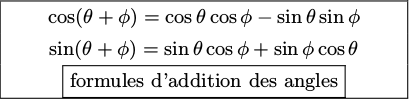
\includegraphics[scale=0.4]{images/011.png}\hfill
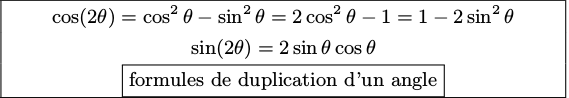
\includegraphics[scale=0.4]{images/012.png}\hfill\end{center}\bigskip\bigskip
$$\overrightarrow{L_0}=\overrightarrow{OM}\times m\overrightarrow{V}$$\\
Ce produit vectoriel implique que $\overrightarrow{OM}$ soit toujours perpendiculaire au vecteur $\overrightarrow{L_0}$ constant.\\
Si $O$ est supposé immobile, une première conséquence est que la trajectoire est contenue dans un plan, perpendiculaire à $\overrightarrow{L_0}$.


% ------------------------------------------------------------------------------------------------------ %
% ------------------------------------------------------------------------------------------------------ %



% ------------------------------------------------------------------------------------------------------ %
% ------------------------------------------------------------------------------------------------------ %


\chapter{Moment d'inertie}
\section{Inertie}
\subsection{Définition}
L'inertie d'un système est définie par $$I=\sum_{i=1}^{N}m_ir_i{}^2$$
avec $I$ l'inertie totale d'un système de masse en $kg\cdot m^2$, $m_i$ une masse ponctuelle, $r_i$ la distance entre l'axe de rotation et la masse ponctuelle $m_i$ et $N$ le nombre de masses ponctuelles.

\section{Énergie}
\subsection{Énergie cinétique de translation}
L'énergie cinétique de translation est définie par $$K=\frac{1}{2}mv^2$$
avec $K$ l'énergie cinétique de translation en Joules, $m$ la masse de l'objet en $Kg$ et $v$ la vitesse de l'objet en $m\cdot s^{-1}$.

\subsection{Énergie cinétique de rotation}
L'énergie cinétique de rotation peut s'écrire $$K=\frac{1}{2}I\omega^2$$
avec $K$ l'énergie cinétique de l'objet en rotation en Joules, $I$ l'inertie de l'objet en rotation autour d'un axe en $Kg\cdot m^2$ et $\omega$ la vitesse angulaire de l'objet en $\rad\cdot s^{-1}$.

\subsection{Démonstration}
$$\begin{array}{rcl} K&=&\displaystyle\sum_{i=1}^{N}K_i \\\\
&=&\displaystyle\sum_{i=1}^N\frac{1}{2}m_iv_i{}^2\\\\
&=&\displaystyle\sum_{i=1}^N\frac{1}{2}m_i(r_i\omega_i)^2 \\\\
&=&\displaystyle\sum_{i=1}^N\frac{1}{2} m_ir_i{}^2\omega^2 \\\\
&=&\frac{1}{2}\omega^2\displaystyle\sum_{i=1}^Nm_ir_i{}^2 \\\\
&=&\frac{1}{2}\omega^2\displaystyle\sum_{i=1}^NI_i \\\\
&=&\frac{1}{2}I\omega^2
\end{array}$$

\section{Moment d'inertie}
\subsection{Cylindre}
\subsubsection{Cylindre creux}


\subsubsection{Cylindre plein}


\subsection{Sphère}
\subsubsection{Sphère creuse}


\subsubsection{Sphère pleine}


\subsection{Tige}
\subsubsection{Rotation centrale}


\subsubsection{Rotation par une extrémité}








\end{document}